\chapter[Metodologia]{Metodologia}

\section{Metodologia de Desenvolvimento de Software}

Um processo ou metodologia de desenvolvimento de software é uma coleção de atividades e resultados relacionados que auxiliam na criação de software. Por exemplo, análise e codificação de requisitos são duas das muitas atividades associadas. \cite{Soares2004}

Há vários tipos de metodologia de desenvolvimento de software como o Scrum, PMBOK, Kanban, Ágil, Ciclo de Vida Único, Modelo em cascata, entre outras. Cada uma delas possui suas próprias características e abordagens para gerenciamento de projetos, mas todas elas visam ajudar as equipes a entregar projetos de software de qualidade dentro do prazo, orçamento e com as funcionalidades esperadas. Algumas metodologias são mais estruturadas e baseadas em fases, enquanto outras são mais flexíveis e baseadas em fluxo de trabalho, o que torna importante escolher a metodologia mais adequada para o projeto específico. \cite{SilvaAnd2013}

\subsection{Metodologia Ágil}

As metodologias ágeis são um conjunto de abordagens para gerenciamento de projetos que se concentram em fornecer flexibilidade, adaptabilidade e colaboração entre equipes. Elas foram desenvolvidas originalmente para o desenvolvimento de software, mas agora são amplamente utilizadas em muitos outros campos. \cite{Libardi2010}

\subsubsection{Scrum}

Scrum é uma metodologia ágil específica que foi projetada para ajudar equipes a gerenciar projetos de desenvolvimento de software complexos e altamente incertos. Ele se concentra em entregar valor rapidamente e incrementos regulares, enquanto a equipe colabora e se adapta a mudanças no projeto. \cite{STOPA2019}

\subsubsection{Kanban}

Kanban é uma metodologia que se concentra em tornar visível o fluxo de trabalho, limitando o número de tarefas em andamento e permitindo que a equipe se adapte às mudanças de forma flexível. Ele é amplamente utilizado em conjunto com outras metodologias ágeis, como Scrum, para ajudar a equipe a aumentar a eficiência e a entrega de valor. \cite{Lage2008}

\subsection{Metodologia de Desenvolvimento Utilizada}

Kanban e Scrum são ambas metodologias ágeis, mas possuem abordagens diferentes para o gerenciamento de projetos. Enquanto o Scrum é uma metodologia mais estruturada e baseada em sprints, Kanban é uma metodologia mais flexível e baseada no fluxo de trabalho. Ambos têm seus próprios benefícios e podem ser usados de forma complementar para ajudar a equipe a alcançar seus objetivos de projeto. \cite{Kniberg2010}

Sendo assim, o projeto foi desenvolvido utilizando ambas as metodologias, Kanban e Scrum, para que fosse possível atingir os objetivos propostos. O Kanban foi utilizado para gerenciar o fluxo de trabalho, enquanto o Scrum foi utilizado para gerenciar as sprints.

\section{Ferramentas Utilizadas}

\subsection{Gerenciamento do Projeto}

\subsubsection{Trello}

\href{https://trello.com/}{Trello} é uma plataforma que auxilia equipes a organizarem e priorizarem projetos. Utiliza quadros de tarefas, onde cada tarefa é representada por um cartão, que pode ser movido e organizado em listas para indicar o progresso e o estado do projeto. Ele é uma ferramenta útil para gerenciar tarefas do projeto, estabelecer prazos e definir prioridades, além de acompanhar o andamento de cada Sprint.

\subsubsection{Slack}

\href{https://slack.com/}{Slack} é uma ferramenta de comunicação de equipe que permite que as equipes criem canais de bate-papo para discutir projetos, compartilhar arquivos e se comunicar de forma rápida e eficiente.

No contexto do desenvolvimento de software, Slack pode ajudar a equipe a se comunicar de forma mais eficiente e colaborativa, permitindo que desenvolvedores, gerentes de projetos e outros membros da equipe discutam e compartilhem informações de forma rápida e fácil. Ele pode ser usado para discutir problemas técnicos, atribuir tarefas, acompanhar o progresso do projeto e compartilhar arquivos, tudo em um único lugar. Além disso, ele pode ser integrado com outras ferramentas, como o GitHub, o Google Drive e o Trello, para ajudar a equipe a automatizar tarefas e trabalhar de forma mais eficiente.

\subsubsection{Google Drive}

\href{https://www.google.com/intl/pt-br/drive/about.html}{Google Drive} é um serviço de armazenamento e compartilhamento de arquivos na nuvem fornecido pelo Google. Ele permite que os usuários armazenem arquivos, como documentos, fotos e vídeos, e compartilhem esses arquivos com outras pessoas. Ele também oferece recursos de colaboração, como edição em tempo real de documentos, comentários e histórico de versões.

\subsection{Desenvolvimento}

\subsubsection{Figma}

\href{https://www.figma.com/}{Figma} é uma ferramenta de design colaborativo que permite que equipes criem e compartilhem arquivos de design. Ele permite que os usuários criem protótipos de aplicativos e sites, além de permitir que eles compartilhem esses protótipos com outras pessoas para que possam colaborar e fazer comentários. Ele também permite que os usuários criem e compartilhem arquivos de design, como imagens, ícones e paletas de cores, que podem ser usados por outros membros da equipe.

\subsubsection{GitHub e GitHub Actions}

\href{https://github.com/}{GitHub} é uma plataforma de desenvolvimento de software que permite que os desenvolvedores armazenem, rastreiem e colaborem em projetos de código-fonte. Ele é baseado no sistema de controle de versão Git, que permite que os desenvolvedores façam alterações no código e versionem essas alterações, facilitando a colaboração e o controle de versão.

GitHub Actions é uma ferramenta de automação de fluxo de trabalho do GitHub. Ele permite que os desenvolvedores criem scripts de trabalho automatizados, chamados ``Ações'', que podem ser disparados por eventos, como o envio de código para o repositório ou a criação de uma nova issue. Isso permite automatizar tarefas comuns, como compilação, teste e implantação, e integrar com outras ferramentas, como ferramentas de integração contínua e de monitoramento de desempenho.

\subsubsection{Docker}

\href{https://www.docker.com/}{Docker} é uma plataforma de virtualização de aplicativos que permite que os desenvolvedores embalem e distribuam facilmente aplicativos em contêineres. Um contêiner é uma forma de isolamento de sistemas operacionais que permite que um aplicativo seja embalado com todas as suas dependências, bibliotecas e configurações, de forma que possa ser executado de forma consistente em diferentes ambientes.

Docker permite que os desenvolvedores criem e gerenciem contêineres, e que esses contêineres sejam implantados em diferentes ambientes, incluindo computadores locais, nuvens públicas e privadas. Isso permite que os desenvolvedores criem aplicativos de forma mais eficiente e confiável, e que esses aplicativos possam ser executados de forma consistente em diferentes ambientes. Além disso, ele também permite a colaboração entre equipes, e aumenta a segurança, escalabilidade e gerenciamento do aplicativo.

\subsubsection{Visual Studio Code}

\href{https://code.visualstudio.com/}{VSCode (Visual Studio Code)} é um editor de código-fonte desenvolvido pela Microsoft. Ele é uma ferramenta gratuita e de código aberto, que suporta diversas linguagens de programação, incluindo JavaScript, Python, C++, Java e muitas outras. Ele oferece recursos avançados de edição, como sugestão de código, depuração e gerenciamento de versão. Além disso, ele também possui uma ampla variedade de extensões e plugins desenvolvidos pela comunidade, que podem ser usadas para adicionar recursos adicionais, como integração com ferramentas de teste, análise de código e integração com outras ferramentas.

\section{Processo de Desenvolvimento}

\subsection{Cronograma}

\section{Cronograma}

O cronograma foi dividido em 6 fases, sendo que cada fase possui um prazo de 2 semanas. A Figura \ref{fig:cronograma} mostra o cronograma completo do projeto.

\begin{itemize}
    \item Fase 1: Reestruturação do trabalho existente; Levantamento de requisitos; criação do modelo de dados, arquitetura e pacotes.
    \item Fase 2, 3 e 4: Desenvolvimento do sistema.
    \item Fase 5: Correção de bugs e ajustes finais; Análise e coleta de resultados.
    \item Fase 6: Documentação e apresentação do projeto.
\end{itemize}

\begin{figure}[H]
    \centering
    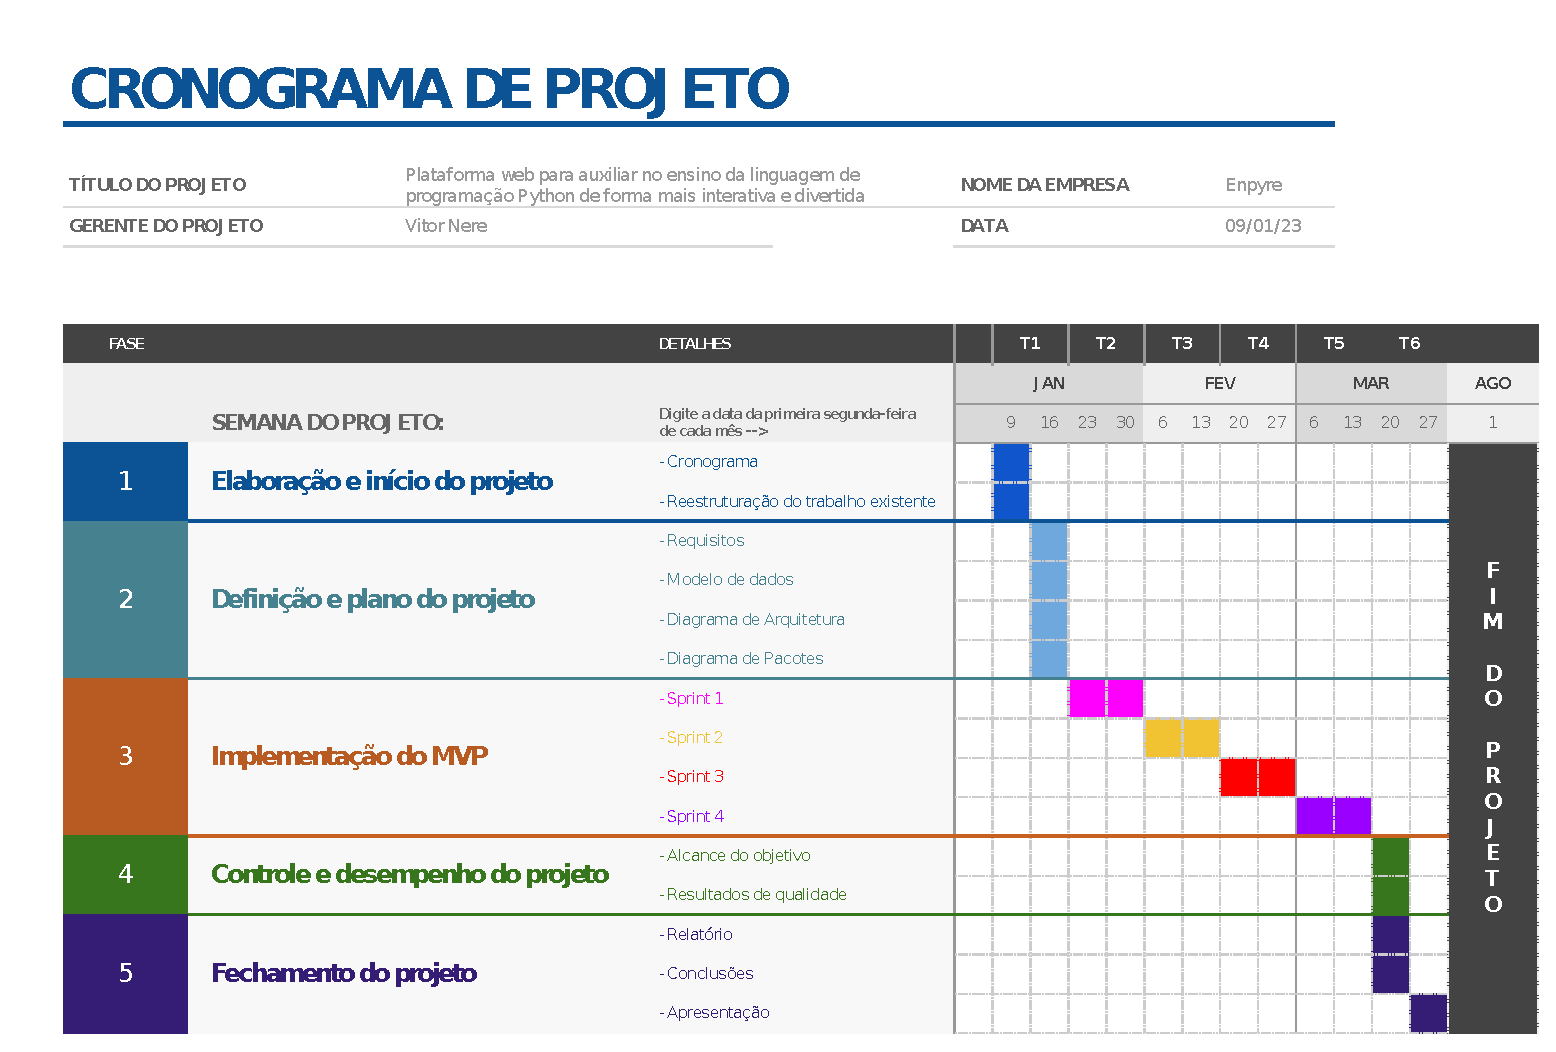
\includegraphics[width=1.1\textwidth]{figuras/cronograma.eps}
    \caption{Cronograma}
    \label{fig:cronograma}
\end{figure}

\subsection{Backlog de desenvolvimento}

O backlog de desenvolvimento foi definido na Fase 1 do cronograma, e é composto por 3 pacotes, sendo que cada pacote possui um conjunto de tarefas. A Figura \ref{fig:backlog} mostra o backlog de desenvolvimento completo do projeto.

\begin{figure}[H]
    \centering
    \includegraphics[width=1\textwidth]{figuras/backlog.eps}
    \caption{Backlog de desenvolvimento}
    \label{fig:backlog}
\end{figure}